% PIDL-ESQ-001 - Esquema eletrico da camara termica PIDlampada - Rev. D
% Versao em LaTeX (circuitikz) do desenho gerado por esquema_eletrico.py.
% Compilar:  pdflatex esquema_eletrico.tex   (duas vezes, por causa do remember picture)
\documentclass{article}
\usepackage[a3paper,landscape,margin=0mm]{geometry}
\usepackage[utf8]{inputenc}
\usepackage[T1]{fontenc}
\usepackage{textcomp}
\usepackage[scaled=0.92]{helvet}
\renewcommand{\familydefault}{\sfdefault}
\usepackage[siunitx,american,RPvoltages]{circuitikz}
\usetikzlibrary{shapes.symbols,shapes.geometric,calc,positioning}
\usepackage{array,tabularx,colortbl,xcolor}
\pagestyle{empty}
\setlength{\parindent}{0pt}
\definecolor{cinza}{HTML}{EEEEEE}
\definecolor{tinta}{HTML}{333333}
\renewcommand{\arraystretch}{1.18}
\ctikzset{bipoles/length=8mm, tripoles/mos style/arrows}
\tikzset{
  rot/.style={font=\scriptsize, align=left, inner sep=1pt},
  rotr/.style={font=\scriptsize, align=right, inner sep=1pt},
  nota/.style={font=\tiny, align=left, text=tinta, inner sep=1pt},
  rede/.style={draw, signal, signal to=east, signal from=west, font=\tiny, inner sep=1.2pt, minimum height=3.4mm, minimum width=16mm},
  redeL/.style={draw, signal, signal to=west, signal from=east, font=\tiny, inner sep=1.2pt, minimum height=3.4mm, minimum width=16mm},
  rev/.style={draw, isosceles triangle, isosceles triangle apex angle=60, shape border rotate=90, inner sep=0.4pt,
              minimum size=3.6mm, font=\tiny\bfseries},
}
% \bloco{x}{y}{w}{h}{titulo}: quadro com titulo, x/y = canto superior esquerdo em mm (como na prancha)
\newcommand{\bloco}[5]{%
  \draw[line width=0.25mm] (#1,297-#2-#4) rectangle (#1+#3,297-#2);
  \node[anchor=north west, draw, line width=0.25mm, fill=white, font=\footnotesize\bfseries, inner sep=1.4mm]
    at (#1,297-#2) {#5};}
% \caixa{x}{y}{w}{h}{titulo}{conteudo}: quadro com tabela/texto
\newcommand{\caixa}[6]{%
  \bloco{#1}{#2}{#3}{#4}{#5}
  \node[anchor=north west, inner sep=0] at (#1+3,297-#2-8.5) {\begin{minipage}[t]{\dimexpr #3mm-6mm\relax}\scriptsize #6\end{minipage}};}
\newcommand{\lab}[3]{\node[font=\scriptsize, align=left, inner sep=0.8pt, anchor=#2] at (#1) {#3};}
\newcommand{\motor}[2]{\draw (#1,#2) circle (3.3) node {\footnotesize M};}
\newcommand{\gnd}[1]{\node[ground] at (#1) {};}
\begin{document}
\begin{tikzpicture}[remember picture, overlay, x=1mm, y=1mm, shift={(current page.south west)}, font=\scriptsize]
\draw[line width=0.7mm] (20,10) rectangle (410,287);
\draw[line width=0.35mm] (25,15) rectangle (405,282);
\draw[line width=0.25mm] (72.50,282) -- (72.50,287) (72.50,10) -- (72.50,15);
\draw[line width=0.25mm] (120.00,282) -- (120.00,287) (120.00,10) -- (120.00,15);
\draw[line width=0.25mm] (167.50,282) -- (167.50,287) (167.50,10) -- (167.50,15);
\draw[line width=0.25mm] (215.00,282) -- (215.00,287) (215.00,10) -- (215.00,15);
\draw[line width=0.25mm] (262.50,282) -- (262.50,287) (262.50,10) -- (262.50,15);
\draw[line width=0.25mm] (310.00,282) -- (310.00,287) (310.00,10) -- (310.00,15);
\draw[line width=0.25mm] (357.50,282) -- (357.50,287) (357.50,10) -- (357.50,15);
\node[font=\scriptsize] at (48.75,284.5) {1}; \node[font=\scriptsize] at (48.75,12.5) {1};
\node[font=\scriptsize] at (96.25,284.5) {2}; \node[font=\scriptsize] at (96.25,12.5) {2};
\node[font=\scriptsize] at (143.75,284.5) {3}; \node[font=\scriptsize] at (143.75,12.5) {3};
\node[font=\scriptsize] at (191.25,284.5) {4}; \node[font=\scriptsize] at (191.25,12.5) {4};
\node[font=\scriptsize] at (238.75,284.5) {5}; \node[font=\scriptsize] at (238.75,12.5) {5};
\node[font=\scriptsize] at (286.25,284.5) {6}; \node[font=\scriptsize] at (286.25,12.5) {6};
\node[font=\scriptsize] at (333.75,284.5) {7}; \node[font=\scriptsize] at (333.75,12.5) {7};
\node[font=\scriptsize] at (381.25,284.5) {8}; \node[font=\scriptsize] at (381.25,12.5) {8};
\draw[line width=0.25mm] (20,237.50) -- (25,237.50) (405,237.50) -- (410,237.50);
\draw[line width=0.25mm] (20,193.00) -- (25,193.00) (405,193.00) -- (410,193.00);
\draw[line width=0.25mm] (20,148.50) -- (25,148.50) (405,148.50) -- (410,148.50);
\draw[line width=0.25mm] (20,104.00) -- (25,104.00) (405,104.00) -- (410,104.00);
\draw[line width=0.25mm] (20,59.50) -- (25,59.50) (405,59.50) -- (410,59.50);
\node[font=\scriptsize] at (22.5,259.75) {A}; \node[font=\scriptsize] at (407.5,259.75) {A};
\node[font=\scriptsize] at (22.5,215.25) {B}; \node[font=\scriptsize] at (407.5,215.25) {B};
\node[font=\scriptsize] at (22.5,170.75) {C}; \node[font=\scriptsize] at (407.5,170.75) {C};
\node[font=\scriptsize] at (22.5,126.25) {D}; \node[font=\scriptsize] at (407.5,126.25) {D};
\node[font=\scriptsize] at (22.5,81.75) {E}; \node[font=\scriptsize] at (407.5,81.75) {E};
\node[font=\scriptsize] at (22.5,37.25) {F}; \node[font=\scriptsize] at (407.5,37.25) {F};
\draw[line width=0.7mm] (210,5) -- (210,15) (210,282) -- (210,292) (15,148.5) -- (25,148.5) (405,148.5) -- (415,148.5);
\node[anchor=south west, font=\tiny, text=tinta] at (20,3) {PIDL-ESQ-001 $\cdot$ REV. D $\cdot$ FOLHA 1/3};
\draw[line width=0.6mm] (268,15) rectangle (405,73);
\foreach \yy in {4.6,9.3} \draw[line width=0.25mm] (268,73-\yy) -- (405,73-\yy);
\foreach \xx in {22,97,113} \draw[line width=0.25mm] (268+\xx,73) -- (268+\xx,59);
\node[font=\tiny\bfseries] at (327.5,70.7) {NOME}; \node[font=\tiny\bfseries] at (373,70.7) {SIGLA};
\node[font=\tiny\bfseries] at (393,70.7) {DATA};
\foreach \yy/\rr in {7/ELABORADO,11.65/APROVADO} {
  \node[font=\tiny\bfseries, anchor=west] at (269.5,73-\yy) {\rr};
  \node[font=\scriptsize, anchor=west] at (292,73-\yy) {Gabriel Marques};
  \node[font=\scriptsize] at (373,73-\yy) {GM}; \node[font=\scriptsize] at (393,73-\yy) {11/10/2026};}
\draw[line width=0.4mm] (268,59) -- (405,59);
\node[anchor=north west, align=left, inner sep=0] at (270,57.5) {\tiny\color{tinta} PROJETO PIDlampada\\[0.6mm]
  \large\bfseries CÂMARA TÉRMICA COM CONTROLE PWM\\[0.4mm] \footnotesize ESQUEMA ELÉTRICO $\cdot$ POTÊNCIA};
\draw[line width=0.25mm] (268,41) -- (405,41);
\node[anchor=west, font=\tiny] at (270,37.5) {UNIP $\cdot$ ENGENHARIA DE COMPUTAÇÃO $\cdot$ PROJETO INTEGRADOR 2026};
\node[anchor=east, font=\tiny] at (403,37.5) {SÃO JOSÉ DOS CAMPOS - SP};
\draw[line width=0.4mm] (268,34) -- (405,34);
\foreach \x in {38,52,70,88,104} \draw[line width=0.25mm] (268+\x,34) -- (268+\x,15);
\foreach \x/\r in {2/Nº DO DESENHO,40/REV.,54/FOLHA,72/ESCALA,90/FORMATO,106/DATA}
  \node[anchor=north west, font=\tiny, text=tinta] at (268+\x,33) {\r};
\node[font=\large\bfseries] at (287,23) {PIDL-ESQ-001};
\node[font=\Large\bfseries] at (313,23) {D};
\node[font=\normalsize] at (329,23) {1 / 3};
\node[font=\normalsize] at (347,23) {S/ ESC.};
\node[font=\normalsize] at (364,23) {A3};
\node[font=\normalsize] at (388.5,23) {11/10/2026};
\node[anchor=north west, inner sep=0] at (268,282) {\scriptsize\setlength{\tabcolsep}{1.2mm}\begin{tabularx}{137mm}{|>{\centering\arraybackslash}p{6mm}|X|>{\centering\arraybackslash}p{15mm}|>{\centering\arraybackslash}p{7mm}|}\hline
\multicolumn{4}{|c|}{\bfseries REVISÕES}\\\hline
\bfseries\tiny REV. & \centering\bfseries\tiny DESCRIÇÃO & \bfseries\tiny DATA & \bfseries\tiny RESP.\\\hline
\bfseries A & Release inicial. & 10/10/2026 & GM\\\hline
\bfseries B & Cooler M1 (Q2, D3, C6, R9, R10). Display DS1 TM1637 (C10). LM35DZ TS1 no lugar do DS18B20 (C8, R11, C9). Entrada ATX = J1. Removidos R1, R8, LED1. & 11/10/2026 & GM\\\hline
\bfseries C & Manta H1 30 W com Q3, R12, R13 e TH2. TH1 KSD301 10 A. F1 6,3 A, D1 SB560, SW1 10 A. GPIO27 = HEAT\_GATE. & 11/10/2026 & GM\\\hline
\bfseries D & Câmara de policarbonato 25 cm (PIDL-MEC-001): 5 lâmpadas, manta 80 W com Q3 IRLB8721, cooler 80 mm e ventoinha de circulação M2 (C11). Cadeia de segurança TH1 85 °C + TH2 120 °C na bobina do relé K1 (D5), que gera +12V\_TH. Q4 IRF4905 no lugar do D1 (R14, D4). F1 15 A, SW1 15 A, C1 2200 \textmu{}F, BT1 3S2P. Desenho em 3 folhas. & 11/10/2026 & GM\\\hline
\end{tabularx}};
\bloco{27}{17}{156}{53}{[1] ENTRADA $\cdot$ SELEÇÃO DE FONTE $\cdot$ PROTEÇÃO}
\bloco{27}{72}{156}{68}{[7] VENTILAÇÃO $\cdot$ EXAUSTÃO E CIRCULAÇÃO}
\bloco{27}{142}{156}{66}{[9] MANTA DE AQUECIMENTO (LOW-SIDE)}
\bloco{185}{60}{220}{70}{[10] CADEIA DE SEGURANÇA TÉRMICA}
\bloco{185}{132}{110}{92}{[6] LÂMPADAS (LOW-SIDE)}
\bloco{297}{132}{108}{46}{[2] REGULAÇÃO 12 V $\rightarrow$ 5 V}
% [1] ENTRADA - SELECAO DE FONTE - PROTECAO   (quadro 156 x 53)
\begin{scope}[shift={(27,227)}]
  \node[spdt, xscale=-1] (sw) at (50,33) {};
  \lab{50,41}{south}{SW1 15 A}  \node[rev] at (41,42.5) {D};
  \node[redeL, anchor=east] (j1) at ($(sw.out 1)+(-14,0)$) {J1 ATX +12 V};
  \draw (j1.east) -- (sw.out 1);
  \draw (30,8) node[ground]{} to[battery1] (30,22) |- (sw.out 2);
  \lab{27,15}{east}{BT1 3S2P 18650\\12,6 V máx.\\BMS $\geq$ 15 A}  \node[rev] at (24,25) {D};
  \draw (sw.in) -- (58,33) to[fuse] (70,33) -- (74,33);
  \lab{64,36.5}{south}{F1 15 A}  \lab{64,29.5}{north}{lâmina retard.}  \node[rev] at (64,43.5) {D};
  \node[pmos, rotate=-90, xscale=-1] (q4) at (81,33) {};
  \draw (74,33) -- (q4.D);
  \lab{81,39.5}{south}{Q4 IRF4905}  \node[rev] at (92.5,42) {D};
  \draw (q4.G) -- (81,22) coordinate (g4) to[R] (81,9) node[ground]{};
  \lab{79,15.5}{east}{R14\\10 k\ensuremath{\Omega}}
  \draw (g4) -- (89,22) to[zDo] (89,33);
  \lab{92,27.5}{west}{D4\\15 V}
  \draw (q4.S) -- (89,33) -- (146,33) -- (146,36); \node[vcc] at (146,36) {}; \lab{146,40}{south}{+12 V PROT}
  \draw (102,12) to[zDo] (102,33);   \lab{105,22.5}{west}{D2\\SMBJ15A}
  \draw (118,33) to[eC] (118,12);    \lab{121,22.5}{west}{C1\\2200 \textmu F\\25 V}  \node[rev] at (118,39) {D};
  \draw (134,33) to[C] (134,12);     \lab{137,22.5}{west}{C2\\100 nF}
  \draw (102,12) -- (134,12); \draw (118,12) node[ground]{};
  \foreach \p in {(89,33),(102,33),(118,33),(134,33),(81,22),(118,12)} \fill \p circle (0.55);
  \node[nota, anchor=north west] at (92,8) {Q4: na polaridade certa conduz com 20 m\ensuremath{\Omega} ($\sim$1,7 W a 9 A);\\invertida, fica cortado. Um Schottky dissiparia $\sim$5 W.};
\end{scope}

% [7] VENTILACAO - EXAUSTAO E CIRCULACAO   (quadro 156 x 68)
\begin{scope}[shift={(27,157)}]
  \draw (46,49) -- (46,53); \node[vcc] at (46,53) {}; \lab{46,57}{south}{+12 V PROT}
  \motor{46}{40}  \draw (46,49) -- (46,43.3) (46,36.7) -- (46,30);
  \lab{41,40}{east}{M1 exaustão\\80 mm $\cdot$ 12 V\\0,15 A}  \node[rev] at (31,50) {D};
  \draw (46,30) -- (60,30) to[sD] (60,49) -- (46,49);
  \lab{63.5,40}{west}{D3 SS14\\roda livre}
  \draw (60,49) -- (82,49) to[C] (82,30) -- (60,30);
  \lab{85,40}{west}{C6\\100 nF}
  \foreach \p in {(46,49),(60,49),(46,30),(60,30)} \fill \p circle (0.55);
  \node[nmos, anchor=D] (q2) at (46,30) {}; \draw (q2.S) node[ground]{};
  \lab{50,21}{west}{Q2 IRLZ44N\\(alt. AO3400)}
  \draw (q2.G) -- ++(-12,0) coordinate (g2) to[R] ++(-14,0) coordinate (t2);
  \lab{$(g2)+(-7,2.8)$}{south}{R9 100 \ensuremath{\Omega}}
  \node[redeL, anchor=east] at (t2) {FAN\_GATE};
  \draw (g2) to[R] ++(0,-13) node[ground]{}; \fill (g2) circle (0.55);
  \lab{$(g2)+(-2,-6.5)$}{east}{R10\\10 k\ensuremath{\Omega}}
  \node[nota, anchor=north west] at (72,12) {Motor = carga INDUTIVA. Fora da cadeia do K1: em sobretemperatura\\as ventoinhas continuam. PWM 25 kHz, LEDC canal 2, rotação mínima 30 \%.};
  \draw (124,49) -- (124,53); \node[vcc] at (124,53) {}; \lab{124,57}{south}{+12 V PROT}
  \motor{124}{40}  \draw (124,49) -- (124,43.3) (124,36.7) -- (124,30) -- (124,27) node[ground]{};
  \draw (124,49) -- (140,49) to[C] (140,30) -- (124,30);
  \lab{143,40}{west}{C11\\100 nF}
  \foreach \p in {(124,49),(124,30)} \fill \p circle (0.55);
  \lab{119,40}{east}{M2 circulação\\60 mm $\cdot$ 12 V\\sempre ligada}  \node[rev] at (108,50) {D};
  \node[nota, anchor=north west] at (104,22) {Sopra ao longo das aletas, sob a\\prateleira: espalha o calor da manta.};
\end{scope}

% [9] MANTA DE AQUECIMENTO (LOW-SIDE)   (quadro 156 x 66)
\begin{scope}[shift={(27,89)}]
  \node[redeL, anchor=east] at (52,49) {+12V\_TH};
  \draw (52,49) -- (60,49) to[R] (60,33);
  \lab{63,41}{west}{H1 manta de silicone\\200 $\times$ 200 mm\\12 V $\cdot$ 80 W $\cdot$ 1,8 \ensuremath{\Omega}}  \node[rev] at (54,39) {D};
  \node[nmos, anchor=D] (q3) at (60,33) {}; \draw (q3.S) node[ground]{};
  \lab{64,24}{west}{Q3 IRLB8721\\8,7 m\ensuremath{\Omega} @ 4,5 V}  \node[rev] at (92,26) {D};
  \draw (q3.G) -- ++(-12,0) coordinate (g3) to[R] ++(-14,0) coordinate (t3);
  \lab{$(g3)+(-7,2.8)$}{south}{R12 150 \ensuremath{\Omega}}
  \node[redeL, anchor=east] at (t3) {HEAT\_GATE};
  \draw (g3) to[R] ++(0,-13) node[ground]{}; \fill (g3) circle (0.55);
  \lab{$(g3)+(-2,-6.5)$}{east}{R13\\10 k\ensuremath{\Omega}}
  \node[nota, anchor=north west] at (106,52) {Carga RESISTIVA: sem diodo de roda livre.\\Mesmo comando das lâmpadas (LEDC canal 1,\\mesmo timer do canal 0).\\6,7 A: Q3 dissipa $\sim$0,4 W.};
  \node[nota, anchor=north west] at (106,30) {Manta colada sob dois dissipadores\\aletados; isolante embaixo; prateleira\\perfurada por cima (nota 9).};
\end{scope}

% [10] CADEIA DE SEGURANCA TERMICA   (quadro 220 x 70)
\begin{scope}[shift={(185,167)}]
  \draw (80,54) -- (80,57); \node[vcc] at (80,57) {}; \lab{80,61}{south}{+12 V PROT}
  \draw (80,54) to[ncs] (80,44) to[ncs] (80,34) -- (80,32) coordinate (k1a) to[cute inductor] (80,18) coordinate (k1b) -- (80,15) node[ground]{};
  \lab{84,49}{west}{TH1 KSD301 85 °C $\cdot$ NF\\no ar, perto do teto}
  \lab{84,39}{west}{TH2 KSD301 120 °C $\cdot$ NF\\no dissipador}  \node[rev] at (72,39) {D};
  \lab{84,25}{west}{K1 relé automotivo\\12 V / 30 A (bobina)}
  \draw (k1b) -- (66,18) to[D] (66,32) -- (k1a);
  \lab{62.5,25}{east}{D5\\1N4007}  \node[rev] at (58,34) {D};
  \fill (k1a) circle (0.55); \fill (k1b) circle (0.55);
  \draw[dashed] (118,25) -- (144,25) -- (144,40.5) -- (147.5,40.5);
  \draw (150,50) -- (150,53); \node[vcc] at (150,53) {}; \lab{150,57}{south}{+12 V PROT}
  \draw (150,50) to[nos] (150,32) -- (150,24) -- (156,24);
  \lab{153,43}{west}{K1\\contato NA}
  \node[rede, anchor=west] at (156,24) {+12V\_TH};
  \node[nota, anchor=north west] at (174,58) {Qualquer termostato que abra\\solta K1: lâmpadas e manta\\ficam sem energia. Ventoinhas,\\ESP32 e display continuam.\\D5: a bobina é INDUTIVA.};
\end{scope}

% [6] LAMPADAS (LOW-SIDE)   (quadro 110 x 92)
\begin{scope}[shift={(185,73)}]
  \node[redeL, anchor=east] at (26,76) {+12V\_TH};
  \foreach \i in {0,...,4} {
    \draw (34,76-9*\i) to[lamp] (62,76-9*\i);
    \pgfmathtruncatemacro{\n}{\i+1}
    \node[font=\scriptsize] at (48,80.6-9*\i) {EL\n};
  }
  \foreach \i in {0,...,3} {\fill (34,76-9*\i) circle (0.55); \fill (62,76-9*\i) circle (0.55);}
  \draw (26,76) -- (34,76) -- (34,40); \draw (62,76) -- (62,30);
  \node[rev] at (70,54) {D};
  \node[nota, anchor=north west] at (70,82) {5 $\times$ W5W 12 V / 5 W\\25 W $\cdot$ 2,1 A total\\carga RESISTIVA:\\sem diodo de roda livre};
  \node[nmos, anchor=D] (q1) at (62,30) {}; \draw (q1.S) node[ground]{};
  \lab{66,21}{west}{Q1 IRLZ44N\\logic-level}
  \draw (q1.G) -- ++(-12,0) coordinate (g1) to[R] ++(-14,0) coordinate (t1);
  \lab{$(g1)+(-7,2.8)$}{south}{R6 150 \ensuremath{\Omega}}
  \node[redeL, anchor=east] at (t1) {PWM\_GATE};
  \draw (g1) to[R] ++(0,-13) node[ground]{}; \fill (g1) circle (0.55);
  \lab{$(g1)+(-2,-6.5)$}{east}{R7\\10 k\ensuremath{\Omega}}
\end{scope}

% [2] REGULACAO 12 V -> 5 V   (quadro 108 x 46)
\begin{scope}[shift={(297,119)}]
  \draw (14,28) -- (14,31); \node[vcc] at (14,31) {}; \lab{14,34.5}{south}{+12 V PROT}
  \draw (14,28) -- (28,28); \draw (28,10) rectangle (56,32);
  \node[font=\tiny, anchor=west] at (28.6,28) {VIN}; \node[font=\tiny, anchor=west] at (28.6,14) {GND};
  \node[font=\tiny, anchor=east] at (55.4,28) {VOUT}; \node[font=\tiny, anchor=east] at (55.4,14) {GND};
  \node[font=\scriptsize, align=center] at (42,21) {U1\\MP1584 / LM2596\\buck 12 $\rightarrow$ 5 V $\cdot$ 3 A};
  \draw (28,14) -- (22,14) -- (22,9) node[ground]{};
  \draw (56,28) -- (98,28) -- (98,31); \node[vcc] at (98,31) {}; \lab{98,34.5}{south}{+5 V}
  \draw (68,28) to[eC] (68,12);  \lab{71,20}{west}{C3\\100 \textmu F}
  \draw (84,28) to[C] (84,12);   \lab{87,20}{west}{C4\\10 \textmu F}
  \draw (56,14) -- (60,14) -- (60,12) -- (84,12); \draw (68,12) node[ground]{};
  \foreach \p in {(68,28),(84,28),(68,12)} \fill \p circle (0.55);
\end{scope}

\caixa{185}{17}{81}{41}{LEGENDA}{\begin{tikzpicture}[x=1mm,y=1mm]
\node[rev] at (3,0) {D}; \node[anchor=west, font=\scriptsize] at (8,0) {alteração desta revisão};
\node[redeL, minimum width=8mm] at (6,-7) {}; \node[anchor=west, font=\scriptsize] at (16,-7) {etiqueta de rede (liga pelo nome)};
\node[ground] at (4,-12.5) {}; \node[anchor=west, font=\scriptsize] at (10,-14) {terra comum};
\draw (0,-21) -- (8,-21) (4,-21) -- (4,-18); \fill (4,-21) circle (0.55); \node[anchor=west, font=\scriptsize] at (10,-21) {junção};
\end{tikzpicture}}
\caixa{27}{210}{156}{70}{REDES DE ALIMENTAÇÃO}{\begin{tabularx}{\linewidth}{|p{18mm}|X|X|p{18mm}|}\hline\rowcolor{cinza}\bfseries\tiny REDE & \bfseries\tiny ORIGEM & \bfseries\tiny CARGAS & \bfseries\tiny CORRENTE\\\hline
+12 V PROT & J1 ou BT1, via SW1, F1 e Q4 & K1 e cadeia TH1/TH2, M1, M2, U1, R2/R3 & $\approx$ 9,1 A máx.\\\hline
+12V\_TH & contato NA do K1 & EL1-EL5 (25 W), H1 (80 W) & $\approx$ 8,8 A máx.\\\hline
+5 V & U1 (buck) & U2 (VIN), TS1 & $\approx$ 0,3 A pico\\\hline
+3V3 & regulador da placa U2 & DS1 & $\leq$ 30 mA\\\hline
\end{tabularx}\\[1.5mm]Fonte: ATX $\geq$ 300 W com 12 V $\geq$ 12 A. A bateria 3S2P mantém 45 °C por \textasciitilde{}1,5 h.}
\caixa{297}{180}{108}{42}{FOLHAS DESTE DESENHO}{\begin{enumerate}\setlength{\itemsep}{1mm}\item Potência: blocos [1] [2] [6] [7] [9] [10]\item Controle e medição: blocos [3] [4] [5] [8]\item Pinagem, notas de projeto e materiais\end{enumerate}}
\caixa{185}{226}{81}{54}{CONDUTORES}{\begin{tabularx}{\linewidth}{|X|p{13mm}|}\hline\rowcolor{cinza}\bfseries\tiny CIRCUITO & \bfseries\tiny SEÇÃO\\\hline
Entrada, K1, +12V\_TH, EL1-EL5, H1, Q1, Q3, Q4 & 1,5 mm$^2$\\\hline
M1, M2, bobina do K1, TH1, TH2, U1 & 0,5 mm$^2$\\\hline
Sinais, TS1 (par trançado), DS1, +5 V & 0,25 mm$^2$\\\hline
\end{tabularx}}
\end{tikzpicture}\null\newpage
\begin{tikzpicture}[remember picture, overlay, x=1mm, y=1mm, shift={(current page.south west)}, font=\scriptsize]
\draw[line width=0.7mm] (20,10) rectangle (410,287);
\draw[line width=0.35mm] (25,15) rectangle (405,282);
\draw[line width=0.25mm] (72.50,282) -- (72.50,287) (72.50,10) -- (72.50,15);
\draw[line width=0.25mm] (120.00,282) -- (120.00,287) (120.00,10) -- (120.00,15);
\draw[line width=0.25mm] (167.50,282) -- (167.50,287) (167.50,10) -- (167.50,15);
\draw[line width=0.25mm] (215.00,282) -- (215.00,287) (215.00,10) -- (215.00,15);
\draw[line width=0.25mm] (262.50,282) -- (262.50,287) (262.50,10) -- (262.50,15);
\draw[line width=0.25mm] (310.00,282) -- (310.00,287) (310.00,10) -- (310.00,15);
\draw[line width=0.25mm] (357.50,282) -- (357.50,287) (357.50,10) -- (357.50,15);
\node[font=\scriptsize] at (48.75,284.5) {1}; \node[font=\scriptsize] at (48.75,12.5) {1};
\node[font=\scriptsize] at (96.25,284.5) {2}; \node[font=\scriptsize] at (96.25,12.5) {2};
\node[font=\scriptsize] at (143.75,284.5) {3}; \node[font=\scriptsize] at (143.75,12.5) {3};
\node[font=\scriptsize] at (191.25,284.5) {4}; \node[font=\scriptsize] at (191.25,12.5) {4};
\node[font=\scriptsize] at (238.75,284.5) {5}; \node[font=\scriptsize] at (238.75,12.5) {5};
\node[font=\scriptsize] at (286.25,284.5) {6}; \node[font=\scriptsize] at (286.25,12.5) {6};
\node[font=\scriptsize] at (333.75,284.5) {7}; \node[font=\scriptsize] at (333.75,12.5) {7};
\node[font=\scriptsize] at (381.25,284.5) {8}; \node[font=\scriptsize] at (381.25,12.5) {8};
\draw[line width=0.25mm] (20,237.50) -- (25,237.50) (405,237.50) -- (410,237.50);
\draw[line width=0.25mm] (20,193.00) -- (25,193.00) (405,193.00) -- (410,193.00);
\draw[line width=0.25mm] (20,148.50) -- (25,148.50) (405,148.50) -- (410,148.50);
\draw[line width=0.25mm] (20,104.00) -- (25,104.00) (405,104.00) -- (410,104.00);
\draw[line width=0.25mm] (20,59.50) -- (25,59.50) (405,59.50) -- (410,59.50);
\node[font=\scriptsize] at (22.5,259.75) {A}; \node[font=\scriptsize] at (407.5,259.75) {A};
\node[font=\scriptsize] at (22.5,215.25) {B}; \node[font=\scriptsize] at (407.5,215.25) {B};
\node[font=\scriptsize] at (22.5,170.75) {C}; \node[font=\scriptsize] at (407.5,170.75) {C};
\node[font=\scriptsize] at (22.5,126.25) {D}; \node[font=\scriptsize] at (407.5,126.25) {D};
\node[font=\scriptsize] at (22.5,81.75) {E}; \node[font=\scriptsize] at (407.5,81.75) {E};
\node[font=\scriptsize] at (22.5,37.25) {F}; \node[font=\scriptsize] at (407.5,37.25) {F};
\draw[line width=0.7mm] (210,5) -- (210,15) (210,282) -- (210,292) (15,148.5) -- (25,148.5) (405,148.5) -- (415,148.5);
\node[anchor=south west, font=\tiny, text=tinta] at (20,3) {PIDL-ESQ-001 $\cdot$ REV. D $\cdot$ FOLHA 2/3};
\draw[line width=0.6mm] (268,15) rectangle (405,73);
\foreach \yy in {4.6,9.3} \draw[line width=0.25mm] (268,73-\yy) -- (405,73-\yy);
\foreach \xx in {22,97,113} \draw[line width=0.25mm] (268+\xx,73) -- (268+\xx,59);
\node[font=\tiny\bfseries] at (327.5,70.7) {NOME}; \node[font=\tiny\bfseries] at (373,70.7) {SIGLA};
\node[font=\tiny\bfseries] at (393,70.7) {DATA};
\foreach \yy/\rr in {7/ELABORADO,11.65/APROVADO} {
  \node[font=\tiny\bfseries, anchor=west] at (269.5,73-\yy) {\rr};
  \node[font=\scriptsize, anchor=west] at (292,73-\yy) {Gabriel Marques};
  \node[font=\scriptsize] at (373,73-\yy) {GM}; \node[font=\scriptsize] at (393,73-\yy) {11/10/2026};}
\draw[line width=0.4mm] (268,59) -- (405,59);
\node[anchor=north west, align=left, inner sep=0] at (270,57.5) {\tiny\color{tinta} PROJETO PIDlampada\\[0.6mm]
  \large\bfseries CÂMARA TÉRMICA COM CONTROLE PWM\\[0.4mm] \footnotesize ESQUEMA ELÉTRICO $\cdot$ CONTROLE E MEDIÇÃO};
\draw[line width=0.25mm] (268,41) -- (405,41);
\node[anchor=west, font=\tiny] at (270,37.5) {UNIP $\cdot$ ENGENHARIA DE COMPUTAÇÃO $\cdot$ PROJETO INTEGRADOR 2026};
\node[anchor=east, font=\tiny] at (403,37.5) {SÃO JOSÉ DOS CAMPOS - SP};
\draw[line width=0.4mm] (268,34) -- (405,34);
\foreach \x in {38,52,70,88,104} \draw[line width=0.25mm] (268+\x,34) -- (268+\x,15);
\foreach \x/\r in {2/Nº DO DESENHO,40/REV.,54/FOLHA,72/ESCALA,90/FORMATO,106/DATA}
  \node[anchor=north west, font=\tiny, text=tinta] at (268+\x,33) {\r};
\node[font=\large\bfseries] at (287,23) {PIDL-ESQ-001};
\node[font=\Large\bfseries] at (313,23) {D};
\node[font=\normalsize] at (329,23) {2 / 3};
\node[font=\normalsize] at (347,23) {S/ ESC.};
\node[font=\normalsize] at (364,23) {A3};
\node[font=\normalsize] at (388.5,23) {11/10/2026};
\bloco{27}{17}{104}{132}{[3] CONTROLADOR}
\bloco{133}{17}{165}{84}{[5] MEDIÇÃO ANALÓGICA}
\bloco{300}{17}{105}{95}{[4] SENSOR DE TEMPERATURA}
\bloco{133}{103}{133}{95}{[8] DISPLAY DE TEMPERATURA}
% [3] CONTROLADOR - U2 ESP32 DEVKIT V1   (quadro 104 x 132)
\begin{scope}[shift={(27,148)}]
  \draw[line width=0.3mm] (28,14) rectangle (62,112);
  \node[font=\scriptsize\bfseries] at (45,116) {U2 ESP32 DevKit v1};
  \foreach \y/\p in {105/VIN, 90/3V3, 55/GND, 20/GND} {\node[font=\tiny, anchor=west] at (28.6,\y) {\p}; \draw (28,\y) -- (16,\y);}
  \draw (16,105) -- (16,108); \node[vcc] at (16,108) {}; \lab{16,111.5}{south}{+5 V}
  \draw (16,90) -- (16,93); \node[vcc] at (16,93) {}; \lab{16,96.5}{south}{+3V3}
  \draw (16,55) -- (16,51) node[ground]{}; \draw (16,20) -- (16,16) node[ground]{};
  \foreach \y/\p/\n in {105/GPIO25/PWM\_GATE, 97/GPIO27/HEAT\_GATE, 89/GPIO26/FAN\_GATE, 81/GPIO32/TEMP\_S,
                       73/GPIO34/V\_SENSE, 65/GPIO35/PWR\_OK\_S, 57/GPIO18/DISP\_CLK, 49/GPIO19/DISP\_DIO,
                       41/GPIO33/SETPOINT, 33/GPIO13/BTN\_MODE, 25/GPIO2/LED\_ST} {
    \node[font=\tiny, anchor=east] at (61.4,\y) {\p}; \draw (62,\y) -- (70,\y);
    \node[rede, anchor=west, minimum width=24mm] at (70,\y) {\n};}
  \node[nota, anchor=north west] at (6,9) {GPIO2: LED de status da placa. GPIO33 e GPIO13: reservados.};
\end{scope}

% [5] MEDICAO ANALOGICA   (quadro 165 x 84)
\begin{scope}[shift={(133,196)}]
  \draw (36,64) -- (36,67); \node[vcc] at (36,67) {}; \lab{36,70.5}{south}{+12 V PROT}
  \draw (36,64) to[R] (36,46) coordinate (vs) to[R] (36,28) -- (36,25) node[ground]{};
  \lab{38.5,55}{west}{R2\\100 k\ensuremath{\Omega}}  \lab{38.5,37}{west}{R3\\27 k\ensuremath{\Omega}}
  \draw (vs) -- (56,46) to[C] (56,28) -- (36,28);  \lab{58.5,37}{west}{C5\\100 nF}
  \foreach \p in {(36,46),(36,28),(56,46)} \fill \p circle (0.55);
  \draw (vs) -- (24,46); \node[redeL, anchor=east] at (24,46) {V\_SENSE};
  \node[nota, anchor=north west] at (6,16) {12,6 V $\rightarrow$ 2,68 V no ADC1.\\O ADC2 conflita com o Wi-Fi.};
  \node[redeL, anchor=east] at (100,58) {PWR\_OK (ATX)};
  \draw (100,58) to[R] (118,58) coordinate (po) -- (130,58);  \lab{109,61}{south}{R4 10 k\ensuremath{\Omega}}
  \node[rede, anchor=west] at (130,58) {PWR\_OK\_S};
  \draw (po) to[R] (118,40) -- (118,37) node[ground]{}; \fill (po) circle (0.55);
  \lab{120.5,49}{west}{R5\\20 k\ensuremath{\Omega}}
  \node[nota, anchor=north west] at (96,28) {PWR\_OK do ATX: 5 V $\rightarrow$ 3,3 V.\\Sem ATX fica em 0 V (= bateria).};
\end{scope}

% [4] SENSOR DE TEMPERATURA   (quadro 105 x 95)
\begin{scope}[shift={(300,185)}]
  \draw (70,30) rectangle (95,64); \node[font=\scriptsize, align=center] at (82.5,70) {TS1 LM35DZ\\10 mV/°C};
  \foreach \y/\p in {58/VS, 48/GND, 36/VOUT} {\node[font=\tiny, anchor=west] at (70.6,\y) {\p};}
  \draw (70,58) -- (44,58) -- (44,62); \node[vcc] at (44,62) {}; \lab{44,65.5}{south}{+5 V}
  \draw (56,58) to[C] (56,49) node[ground]{}; \fill (56,58) circle (0.55);  \lab{54,53.5}{east}{C8\\100 nF}
  \draw (70,48) -- (66,48) -- (66,45) node[ground]{};
  \draw (70,36) to[R] (54,36) coordinate (ts) -- (30,36);  \lab{62,39}{south}{R11 75 \ensuremath{\Omega}}
  \node[redeL, anchor=east] at (30,36) {TEMP\_S};
  \draw (ts) to[C] (54,22) node[ground]{}; \fill (ts) circle (0.55);  \lab{56,29}{west}{C9\\1 \textmu F}
  \node[nota, anchor=north west] at (8,14) {Filtro R11 + C9 do datasheet: o LM35 oscila\\com capacitor ligado direto na saída.};
\end{scope}

% [8] DISPLAY DE TEMPERATURA   (quadro 133 x 95)
\begin{scope}[shift={(133,99)}]
  \draw (78,22) rectangle (106,64); \node[font=\scriptsize, align=center] at (92,70) {DS1 TM1637\\4 dígitos};
  \foreach \y/\p in {58/VCC, 44/CLK, 36/DIO, 26/GND} {\node[font=\tiny, anchor=west] at (78.6,\y) {\p};}
  \draw (78,58) -- (52,58) -- (52,62); \node[vcc] at (52,62) {}; \lab{52,65.5}{south}{+3V3}
  \draw (64,58) to[C] (64,50) node[ground]{}; \fill (64,58) circle (0.55);  \lab{62,54}{east}{C10\\100 nF}
  \draw (78,44) -- (46,44); \node[redeL, anchor=east] at (46,44) {DISP\_CLK};
  \draw (78,36) -- (46,36); \node[redeL, anchor=east] at (46,36) {DISP\_DIO};
  \draw (78,26) -- (72,26) -- (72,22) node[ground]{};
  \node[nota, anchor=north west] at (8,14) {VCC em 3,3 V: o ESP32 não tolera 5 V no DIO.};
\end{scope}

\caixa{268}{114}{137}{108}{NOTAS GERAIS}{\footnotesize \begin{enumerate}\setlength{\itemsep}{1.2mm}\item Folha 1: potência. Folha 2: controle e medição. Folha 3: pinagem, notas e materiais.\item Triângulo com "D": incluído ou alterado nesta revisão. Revisões anteriores na tabela da folha 1.\item Etiquetas de rede com o mesmo nome estão interligadas, inclusive entre folhas.\item Todos os símbolos de terra são o mesmo nó: GND do pack, do ATX, do U1 e do U2.\item Resistores 1/4 W 5 \%. Capacitores cerâmicos X7R 50 V. Salvo indicação.\item Malha de potência (+12 V PROT, K1, +12V\_TH, EL1-EL5, H1, Q1, Q3, Q4): fio de 1,5 mm$^2$ (15 A).\item Montagem mecânica, furação e plano de corte da chapa: desenho PIDL-MEC-001.\end{enumerate}}
\caixa{27}{151}{104}{47}{LEGENDA}{\begin{tikzpicture}[x=1mm,y=1mm]
\node[rev] at (3,0) {D}; \node[anchor=west, font=\scriptsize] at (8,0) {alteração desta revisão};
\node[redeL, minimum width=8mm] at (6,-7) {}; \node[anchor=west, font=\scriptsize] at (16,-7) {etiqueta de rede (liga pelo nome)};
\node[ground] at (4,-12.5) {}; \node[anchor=west, font=\scriptsize] at (10,-14) {terra comum};
\draw (0,-21) -- (8,-21) (4,-21) -- (4,-18); \fill (4,-21) circle (0.55); \node[anchor=west, font=\scriptsize] at (10,-21) {junção};
\end{tikzpicture}}
\caixa{27}{200}{239}{80}{INTERLIGAÇÃO DAS REDES}{\begin{tabularx}{\linewidth}{|p{36mm}|p{58mm}|X|p{18mm}|}\hline\rowcolor{cinza}\bfseries\tiny REDE & \bfseries\tiny ORIGEM & \bfseries\tiny DESTINO & \bfseries\tiny FOLHAS\\\hline
PWM\_GATE & [3] U2 GPIO25 & [6] Q1 & 2 $\rightarrow$ 1\\\hline
HEAT\_GATE & [3] U2 GPIO27 & [9] Q3 & 2 $\rightarrow$ 1\\\hline
FAN\_GATE & [3] U2 GPIO26 & [7] Q2 & 2 $\rightarrow$ 1\\\hline
TEMP\_S & [4] TS1 via R11/C9 & [3] U2 GPIO32 & 2\\\hline
V\_SENSE & [5] R2/R3 & [3] U2 GPIO34 & 2\\\hline
PWR\_OK\_S & [5] R4/R5 & [3] U2 GPIO35 & 2\\\hline
DISP\_CLK $\cdot$ DISP\_DIO & [3] U2 GPIO18 $\cdot$ GPIO19 & [8] DS1 & 2\\\hline
+12 V PROT & [1] & [2] [7] [10] $\cdot$ [5] & 1 $\rightarrow$ 1, 2\\\hline
+12V\_TH & [10] contato do K1 & [6] [9] & 1\\\hline
+5 V & [2] U1 & [3] U2 $\cdot$ [4] TS1 & 1 $\rightarrow$ 2\\\hline
+3V3 & [3] U2 & [8] DS1 & 2\\\hline
\end{tabularx}}
\end{tikzpicture}\null\newpage
\begin{tikzpicture}[remember picture, overlay, x=1mm, y=1mm, shift={(current page.south west)}, font=\scriptsize]
\draw[line width=0.7mm] (20,10) rectangle (410,287);
\draw[line width=0.35mm] (25,15) rectangle (405,282);
\draw[line width=0.25mm] (72.50,282) -- (72.50,287) (72.50,10) -- (72.50,15);
\draw[line width=0.25mm] (120.00,282) -- (120.00,287) (120.00,10) -- (120.00,15);
\draw[line width=0.25mm] (167.50,282) -- (167.50,287) (167.50,10) -- (167.50,15);
\draw[line width=0.25mm] (215.00,282) -- (215.00,287) (215.00,10) -- (215.00,15);
\draw[line width=0.25mm] (262.50,282) -- (262.50,287) (262.50,10) -- (262.50,15);
\draw[line width=0.25mm] (310.00,282) -- (310.00,287) (310.00,10) -- (310.00,15);
\draw[line width=0.25mm] (357.50,282) -- (357.50,287) (357.50,10) -- (357.50,15);
\node[font=\scriptsize] at (48.75,284.5) {1}; \node[font=\scriptsize] at (48.75,12.5) {1};
\node[font=\scriptsize] at (96.25,284.5) {2}; \node[font=\scriptsize] at (96.25,12.5) {2};
\node[font=\scriptsize] at (143.75,284.5) {3}; \node[font=\scriptsize] at (143.75,12.5) {3};
\node[font=\scriptsize] at (191.25,284.5) {4}; \node[font=\scriptsize] at (191.25,12.5) {4};
\node[font=\scriptsize] at (238.75,284.5) {5}; \node[font=\scriptsize] at (238.75,12.5) {5};
\node[font=\scriptsize] at (286.25,284.5) {6}; \node[font=\scriptsize] at (286.25,12.5) {6};
\node[font=\scriptsize] at (333.75,284.5) {7}; \node[font=\scriptsize] at (333.75,12.5) {7};
\node[font=\scriptsize] at (381.25,284.5) {8}; \node[font=\scriptsize] at (381.25,12.5) {8};
\draw[line width=0.25mm] (20,237.50) -- (25,237.50) (405,237.50) -- (410,237.50);
\draw[line width=0.25mm] (20,193.00) -- (25,193.00) (405,193.00) -- (410,193.00);
\draw[line width=0.25mm] (20,148.50) -- (25,148.50) (405,148.50) -- (410,148.50);
\draw[line width=0.25mm] (20,104.00) -- (25,104.00) (405,104.00) -- (410,104.00);
\draw[line width=0.25mm] (20,59.50) -- (25,59.50) (405,59.50) -- (410,59.50);
\node[font=\scriptsize] at (22.5,259.75) {A}; \node[font=\scriptsize] at (407.5,259.75) {A};
\node[font=\scriptsize] at (22.5,215.25) {B}; \node[font=\scriptsize] at (407.5,215.25) {B};
\node[font=\scriptsize] at (22.5,170.75) {C}; \node[font=\scriptsize] at (407.5,170.75) {C};
\node[font=\scriptsize] at (22.5,126.25) {D}; \node[font=\scriptsize] at (407.5,126.25) {D};
\node[font=\scriptsize] at (22.5,81.75) {E}; \node[font=\scriptsize] at (407.5,81.75) {E};
\node[font=\scriptsize] at (22.5,37.25) {F}; \node[font=\scriptsize] at (407.5,37.25) {F};
\draw[line width=0.7mm] (210,5) -- (210,15) (210,282) -- (210,292) (15,148.5) -- (25,148.5) (405,148.5) -- (415,148.5);
\node[anchor=south west, font=\tiny, text=tinta] at (20,3) {PIDL-ESQ-001 $\cdot$ REV. D $\cdot$ FOLHA 3/3};
\draw[line width=0.6mm] (268,15) rectangle (405,73);
\foreach \yy in {4.6,9.3} \draw[line width=0.25mm] (268,73-\yy) -- (405,73-\yy);
\foreach \xx in {22,97,113} \draw[line width=0.25mm] (268+\xx,73) -- (268+\xx,59);
\node[font=\tiny\bfseries] at (327.5,70.7) {NOME}; \node[font=\tiny\bfseries] at (373,70.7) {SIGLA};
\node[font=\tiny\bfseries] at (393,70.7) {DATA};
\foreach \yy/\rr in {7/ELABORADO,11.65/APROVADO} {
  \node[font=\tiny\bfseries, anchor=west] at (269.5,73-\yy) {\rr};
  \node[font=\scriptsize, anchor=west] at (292,73-\yy) {Gabriel Marques};
  \node[font=\scriptsize] at (373,73-\yy) {GM}; \node[font=\scriptsize] at (393,73-\yy) {11/10/2026};}
\draw[line width=0.4mm] (268,59) -- (405,59);
\node[anchor=north west, align=left, inner sep=0] at (270,57.5) {\tiny\color{tinta} PROJETO PIDlampada\\[0.6mm]
  \large\bfseries CÂMARA TÉRMICA COM CONTROLE PWM\\[0.4mm] \footnotesize PINAGEM $\cdot$ NOTAS DE PROJETO $\cdot$ LISTA DE MATERIAIS};
\draw[line width=0.25mm] (268,41) -- (405,41);
\node[anchor=west, font=\tiny] at (270,37.5) {UNIP $\cdot$ ENGENHARIA DE COMPUTAÇÃO $\cdot$ PROJETO INTEGRADOR 2026};
\node[anchor=east, font=\tiny] at (403,37.5) {SÃO JOSÉ DOS CAMPOS - SP};
\draw[line width=0.4mm] (268,34) -- (405,34);
\foreach \x in {38,52,70,88,104} \draw[line width=0.25mm] (268+\x,34) -- (268+\x,15);
\foreach \x/\r in {2/Nº DO DESENHO,40/REV.,54/FOLHA,72/ESCALA,90/FORMATO,106/DATA}
  \node[anchor=north west, font=\tiny, text=tinta] at (268+\x,33) {\r};
\node[font=\large\bfseries] at (287,23) {PIDL-ESQ-001};
\node[font=\Large\bfseries] at (313,23) {D};
\node[font=\normalsize] at (329,23) {3 / 3};
\node[font=\normalsize] at (347,23) {S/ ESC.};
\node[font=\normalsize] at (364,23) {A3};
\node[font=\normalsize] at (388.5,23) {11/10/2026};
\node[anchor=north west, inner sep=0] at (27,279) {\begin{minipage}[t]{190mm}\footnotesize{\normalsize\bfseries PINAGEM $\cdot$ U2 ESP32 DEVKIT V1}\\[-1mm]\rule{190mm}{0.4mm}\\[1mm]\begin{tabularx}{\linewidth}{|p{15mm}|p{22mm}|p{17mm}|X|p{8mm}|}\hline\rowcolor{cinza}\bfseries\tiny PINO & \bfseries\tiny REDE & \bfseries\tiny TIPO & \bfseries\tiny FUNÇÃO & \bfseries\tiny REV.\\\hline
GPIO25 & PWM\_GATE & saída & Gate do Q1 (5 lâmpadas) $\cdot$ LEDC canal 0, 500 Hz, 10 bits & A\\\hline
GPIO27 & HEAT\_GATE & saída & Gate do Q3 (manta 80 W) $\cdot$ LEDC canal 1, mesmo timer das lâmpadas & C\\\hline
GPIO26 & FAN\_GATE & saída & Gate do Q2 (cooler 80 mm) $\cdot$ LEDC canal 2, 25 kHz, 8 bits & B\\\hline
GPIO32 & TEMP\_S & analógica & ADC1\_CH4 $\leftarrow$ LM35 via filtro R11/C9 & B\\\hline
GPIO34 & V\_SENSE & analógica & ADC1\_CH6 $\leftarrow$ divisor R2/R3 (tensão do barramento) & A\\\hline
GPIO35 & PWR\_OK\_S & analógica & ADC1\_CH7 $\leftarrow$ divisor R4/R5 (PWR\_OK do ATX) & A\\\hline
GPIO18 & DISP\_CLK & saída & Clock do TM1637 (DS1) & B\\\hline
GPIO19 & DISP\_DIO & bidirecional & Dados do TM1637, dreno aberto com pull-up no módulo & B\\\hline
GPIO2 & — & saída & LED de status da própria placa & B\\\hline
GPIO33 & SETPOINT & analógica & Reservado: potenciômetro de setpoint (só na simulação) & A\\\hline
GPIO13 & BTN\_MODE & entrada & Reservado: botão de modo & C\\\hline
VIN & +5 V & alimentação & Entrada de 5 V vinda do U1 & A\\\hline
3V3 & +3V3 & alimentação & Saída do regulador da placa $\rightarrow$ DS1 & A\\\hline
GND & GND & terra & Terra comum & A\\\hline
\end{tabularx}\\[4mm]{\normalsize\bfseries NOTAS DE PROJETO}\\[-1mm]\rule{190mm}{0.4mm}\begin{enumerate}\setlength{\itemsep}{0.9mm}\item \textbf{Diodos de roda livre só nas cargas indutivas.} Lâmpadas e manta são resistivas e dispensam diodo. O motor do cooler (D3) e a bobina do relé K1 (D5) são indutivos: ao desligar, a corrente do enrolamento precisa de caminho e, sem o diodo, vira um pico de tensão que queima o MOSFET ou o termostato. D3 é Schottky porque o PWM é de 25 kHz.\item \textbf{Ventoinhas fora da cadeia de segurança.} Em sobretemperatura K1 corta lâmpadas e manta e o firmware põe o cooler a 100 \%. Se as ventoinhas também fossem cortadas, a câmara esfriaria só por convecção.\item \textbf{Faixa dividida (split-range).} Um único PI com saída de $-$1 a 1: positivo aciona lâmpadas e manta, negativo aciona o cooler, nunca os dois juntos. O cooler tem rotação mínima de 30 \% e histerese de liga/desliga.\item \textbf{Canais LEDC.} Os canais andam em pares que dividem um timer (0-1, 2-3...). Lâmpadas (0) e manta (1) dividem de propósito o timer de 500 Hz; o cooler fica no canal 2 para os 25 kHz dele não mudarem essa frequência.\item \textbf{LM35 em 5 V.} O LM35 pede de 4 a 30 V. A saída, de 0,25 a 0,70 V na faixa útil, entra no ADC sem divisor. O LM35DZ mede de 0 a 100 °C: o teto de 70 °C no setpoint deixa folga.\item \textbf{TM1637 em 3,3 V.} Os pull-ups do módulo vão no VCC. Com o módulo em 5 V o pino DIO do ESP32 receberia acima do limite.\item \textbf{Proteções da entrada.} Q4 (P-MOSFET) faz a proteção contra inversão: conduz com 20 m\ensuremath{\Omega} na polaridade certa e corta na invertida. D4 limita o VGS. D2 absorve transitórios de hot-plug; F1 é lento para o inrush das lâmpadas frias e do C1. R7, R10 e R13 seguram os gates em 0 V durante o boot.\item \textbf{Compensação de tensão.} Com bateria a tensão cai de 12,6 para \textasciitilde{}10 V. O firmware corrige o duty das lâmpadas e da manta por (12/V)$^2$ e o do cooler por 12/V, medindo V pelo V\_SENSE.\item \textbf{Manta, dissipadores e prateleira.} H1 vai colada sob dois dissipadores aletados, sobre isolante de fibra cerâmica. A ventoinha M2, sempre ligada, sopra o ar pelas aletas; o ar quente sobe pelos furos da prateleira de alumínio perfurado, onde ficam as amostras. Lâmpadas e manta recebem o mesmo comando; o feedforward usa o ganho somado (16 + 50 °C).\item \textbf{Cadeia de segurança.} TH1 (85 °C, no ar) e TH2 (120 °C, no dissipador) em série com a bobina do K1. Qualquer um que abra solta o relé e tira a energia de lâmpadas e manta; o firmware ainda corta tudo acima de 78 °C. Os termostatos só conduzem os \textasciitilde{}80 mA da bobina, não os 8,8 A da carga.\item \textbf{Câmara de policarbonato.} PC compacto cristal de 6 mm (U $\approx$ 3,9 W/m$^2$K) aguenta uso contínuo até \textasciitilde{}115 °C. Câmara de 25 $\times$ 25 $\times$ 25 cm: UA $\approx$ 1,6 W/K e constante de tempo $\approx$ 1000 s, por isso a potência subiu para 105 W. Ver PIDL-MEC-001.\end{enumerate}\end{minipage}};
\node[anchor=north west, inner sep=0] at (223,279) {\begin{minipage}[t]{180mm}\footnotesize{\normalsize\bfseries LISTA DE MATERIAIS (ELÉTRICA)}\\[-1mm]\rule{180mm}{0.4mm}\\[1mm]\begin{tabularx}{\linewidth}{|p{6mm}|p{24mm}|p{7mm}|X|p{31mm}|p{8mm}|}\hline\rowcolor{cinza}\bfseries\tiny ITEM & \bfseries\tiny REF. & \bfseries\tiny QTD. & \bfseries\tiny DESCRIÇÃO & \bfseries\tiny ESPECIFICAÇÃO & \bfseries\tiny REV.\\\hline
1 & BT1 & 1 & Pack 3S2P 18650 (alto dreno) com BMS & 12,6 V $\cdot$ BMS $\geq$ 15 A & $\triangle$D\\\hline
2 & J1 & 1 & Conector ATX (Molex 4 vias), fonte $\geq$ 300 W & 12 V $\geq$ 12 A & $\triangle$D\\\hline
3 & SW1 & 1 & Chave seletora SPDT & 15 A $\cdot$ ATX / bateria & $\triangle$D\\\hline
4 & F1 & 1 & Fusível lâmina + porta-fusível & 15 A retardado & $\triangle$D\\\hline
5 & Q4 & 1 & MOSFET canal P IRF4905 + dissipador & 55 V $\cdot$ 20 m\ensuremath{\Omega} & $\triangle$D\\\hline
6 & D4 & 1 & Diodo zener & 15 V $\cdot$ 0,5 W & $\triangle$D\\\hline
7 & D2 & 1 & Supressor TVS SMBJ15A & 15 V $\cdot$ 600 W & A\\\hline
8 & C1 & 1 & Capacitor eletrolítico & 2200 \textmu{}F $\cdot$ 25 V & $\triangle$D\\\hline
9 & C2, C5, C6, C8, C10, C11 & 6 & Capacitor cerâmico & 100 nF $\cdot$ 50 V & $\triangle$D\\\hline
10 & U1 & 1 & Módulo buck MP1584 / LM2596 & 12 $\rightarrow$ 5 V $\cdot$ 3 A & A\\\hline
11 & C3 $\cdot$ C4 & 2 & Eletrolítico $\cdot$ cerâmico & 100 \textmu{}F $\cdot$ 10 \textmu{}F, 16 V & A\\\hline
12 & U2 & 1 & Placa ESP32 DevKit v1 & 30 pinos & A\\\hline
13 & TH1 & 1 & Termostato bimetálico KSD301 (no ar) & 85 °C $\cdot$ NF & $\triangle$D\\\hline
14 & TH2 & 1 & Termostato bimetálico KSD301 (no dissipador) & 120 °C $\cdot$ NF & $\triangle$D\\\hline
15 & K1 & 1 & Relé automotivo + soquete & 12 V $\cdot$ 30 A $\cdot$ NA & $\triangle$D\\\hline
16 & D5 & 1 & Diodo retificador 1N4007 & 1 A $\cdot$ 1000 V & $\triangle$D\\\hline
17 & EL1-EL5 & 5 & Lâmpada halógena W5W com soquete T10 & 12 V $\cdot$ 5 W & $\triangle$D\\\hline
18 & Q1, Q2 & 2 & MOSFET canal N IRLZ44N (Q2 alt. AO3400) & logic-level & A\\\hline
19 & Q3 & 1 & MOSFET canal N IRLB8721 & 8,7 m\ensuremath{\Omega} @ 4,5 V & $\triangle$D\\\hline
20 & H1 & 1 & Manta de silicone 200 $\times$ 200 mm & 12 V $\cdot$ 80 W $\cdot$ 1,8 \ensuremath{\Omega} & $\triangle$D\\\hline
21 & M1 & 1 & Ventoinha de exaustão 80 $\times$ 80 $\times$ 25 mm & 12 V $\cdot$ 0,15 A & $\triangle$D\\\hline
22 & M2 & 1 & Ventoinha de circulação 60 $\times$ 60 $\times$ 15 mm & 12 V $\cdot$ 0,1 A & $\triangle$D\\\hline
23 & D3 & 1 & Diodo Schottky SS14 (alt. 1N5819) & 1 A $\cdot$ 40 V & B\\\hline
24 & TS1 & 1 & Sensor de temperatura LM35DZ & 10 mV/°C $\cdot$ TO-92 & B\\\hline
25 & C9 & 1 & Capacitor cerâmico & 1 \textmu{}F $\cdot$ 16 V & B\\\hline
26 & DS1 & 1 & Módulo display TM1637 & 4 dígitos com ponto & B\\\hline
27 & R2 $\cdot$ R3 $\cdot$ R5 & 3 & Resistor & 100 k\ensuremath{\Omega} $\cdot$ 27 k\ensuremath{\Omega} $\cdot$ 20 k\ensuremath{\Omega} & A\\\hline
28 & R4, R7, R10, R13, R14 & 5 & Resistor & 10 k\ensuremath{\Omega} & $\triangle$D\\\hline
29 & R6, R12 $\cdot$ R9 $\cdot$ R11 & 4 & Resistor & 150 \ensuremath{\Omega} $\cdot$ 100 \ensuremath{\Omega} $\cdot$ 75 \ensuremath{\Omega} & C\\\hline
\end{tabularx}\\[1mm]Peças mecânicas (chapa de PC, cantoneiras, base de MDF, dobradiças): lista do PIDL-MEC-001. Removidos ao longo das revisões: R1, R8, LED1, DS18B20 (B) e D1 (D, trocado por Q4).\end{minipage}};
\end{tikzpicture}\null
\end{document}
